	
	\begin{minipage}{0.5\linewidth}
		
	\section{Pilz- und Flachdecken}
	
	\textbf{Def.:} unterzugslose Decken, die direkt auf Stützen mit oder ohne Stützenkopfverstärkung (Pilze) gelagert sind. \\
	
	\textbf{Nachteile}
	\begin{itemize}
		
		\item höherer Beton- und Stahlverbrauch
		
		\item grössere Durchbiegung
		
		\item höhere Beanspruchung im Stützenbereich (Durchstanzen)
		
	\end{itemize}

	\end{minipage}
	\begin{minipage}{0.5\linewidth}
		
		
		\textbf{Vorteile}
		\begin{itemize}
			
			\item ebene Betonunterfläche vereinfache Schalung \& Bewehrung verlegen $\rightarrow$ beschleunigt Bauablauf
			
			\item Installationen werden nicht durch Unterzüge behindert $\rightarrow$ Tragwerksplanung kann starten, vor Leitungsführungsplanungabschluss
			
			\item grosse Stützenabstände möglich
			
			\item Flexibilität für spätere Änderungen
			
			\item geringere Konstruktionshöhe 
			
		\end{itemize}			
		
	\end{minipage}



	\begin{minipage}{0.5\linewidth}
		
		\subsection{Tragverhalten}
		
		\begin{wrapfigure}{L}{0.2\linewidth}
			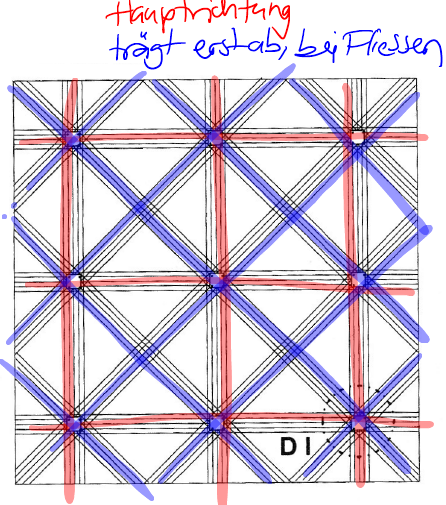
\includegraphics[width=\linewidth]{images/PilzFlach1Lastabtrag.PNG}
		\end{wrapfigure}
	
		Punktgestützte Platten tragen Lasten nicht nur in 2 Richtungen, sondern rotationssymmetrisch um die Stützen ab
		
		\textbf{Modell}
		
		Biegemomente und Querkräfte über 4 Streifen abtragen \\	
		
		
		
		\begin{wrapfigure}{L}{0.3\linewidth}
			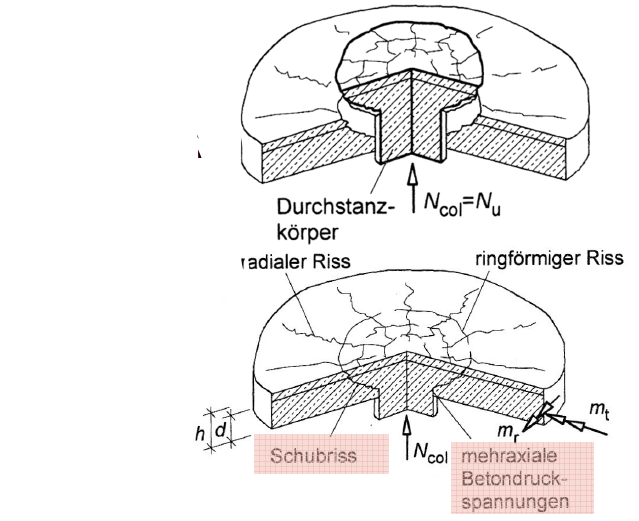
\includegraphics[width=\linewidth]{images/PilzFlach2Schnittkrat.PNG}
		\end{wrapfigure}
	
		1. Radialmomente m$_r$ um Stütze $\rightarrow$ ringförmige Risse \\
		2. Tangentialmomente m$_t$ $\rightarrow$ Biegerisse in Radialrichtung \\
		3. an Unterseite mehraxialer Spannungszustand im Beton $\rightarrow$ Schubrisse \\
		4. Einschnürung der Druckzone $\rightarrow$ Durchstanzversagen
			
	\end{minipage}
	\begin{minipage}{0.5\linewidth}
		
		\subsection{Biegemomente Ermittlung}
		
		\begin{wrapfigure}{L}{0.3\linewidth}
			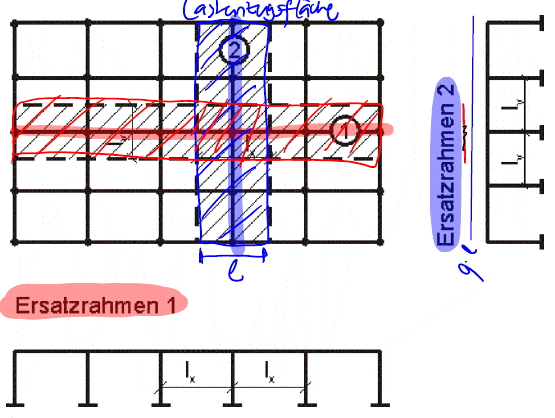
\includegraphics[width=\linewidth, angle=270,origin=c]{images/PilzFlach3Rahmen.PNG}
		\end{wrapfigure}
	
	
	
			1. FEM \\
			2. \textbf{Methode der stellvertretenden Rahmen}

			
				\begin{itemize}
					
					\item gleichmässig verteilte Lasten (nicht für Einzellasten)
					
					\item zwei sich gegenseitig durchdringenden, biegesteif mit den stützen verbundenen Rahmen
					
					\item senkrecht stehende Rahmen haben je die volle Last abzutragen
					
					\item Biegesteifigkeit Stützen gering $\rightarrow$ Annahme: Durchlaufträger
					
					\item ohne Drillmomente, trotzdem statisch sichere Bemessung
					
				\end{itemize}
		
	\end{minipage}

	\begin{minipage}{0.5\linewidth}
		
		\subsection{Durchstanznachweis}
			SIA 261 4.3
		
	\end{minipage}